\documentclass[../Article_Model_Parameters.tex]{subfiles}
\graphicspath{{\subfix{../Figures/}}}
\begin{document}
	
	In recent years, the use of solvents for extracting natural substances from solid materials and liquids has been an area of significant interest for research and development. Supercritical fluids, which exhibit both gas- and liquid-like properties, have proven particularly useful in extraction processes due to their pressure-dependent dissolving power. Supercritical $CO_2$, in particular, is attractive because it is nontoxic, non-flammable, and non-corrosive. Furthermore, its critical point is relatively low compared to other fluids, making it a suitable alternative to traditional extraction techniques.
	
	Various mathematical models have been proposed to describe the extraction of valuable compounds from a fixed biomass bed. However, selecting an appropriate extraction model requires understanding the physical phenomena occurring in the operational unit. Each model has its own set of assumptions and describes different mass transfer mechanisms and equilibrium relationships.
	
	One model proposed by \citet{Reverchon1993} is the hot ball model, which is based on an analogy to heat transfer and describes an extraction process from solid particles containing small quantities of solute where solubility is not a limiting factor. Another model, called the Broken-and-Intact Cell model, was presented by \citet{Sovova1994}. This model describes a system where the outer surfaces of particles have been mechanically interrupted, allowing easy access of solvent to the solute from the broken cells. In contrast, the solute from the intact cells is less accessible due to high mass transfer resistance.
	
	\citet{Reverchon1996} developed a model for fluid-solid extraction, where the oil is treated as a single component, and the extraction process is controlled by internal mass transfer resistance, neglecting external mass transfer. However, this model does not consider the influence of axial dispersion or changes in density and flow rate along the bed.
	
	In this work, the basic governing equations are derived and combine them with the kinetic model suggested by \citet{Reverchon1996} to obtain a general model for the extraction process of the oil from the caraway seed. This model simplifies some of the physical behavior to obtain a control-oriented model. It is assumed that the extraction process operates semi-continuously in a cylindrical vessel. The solvent is first brought to supercritical conditions, pumped through a fixed bed of finely chopped biomass, and the solute is extracted from the biomass. The solvent and solute are then separated in a flush drum, and the extract is collected. The feed flow rate ($F_{in}$) and inlet temperature ($T_{in}$) of the extractor can be measured and manipulated, while the vessel pressure ($P$) can also be measured and manipulated. However, the outlet temperature ($T_{out}$) can only be measured. Figure \ref{fig: SFE_drawing} shows a simplified flow diagram.
	
	\begin{figure}[h!]
		\centering
		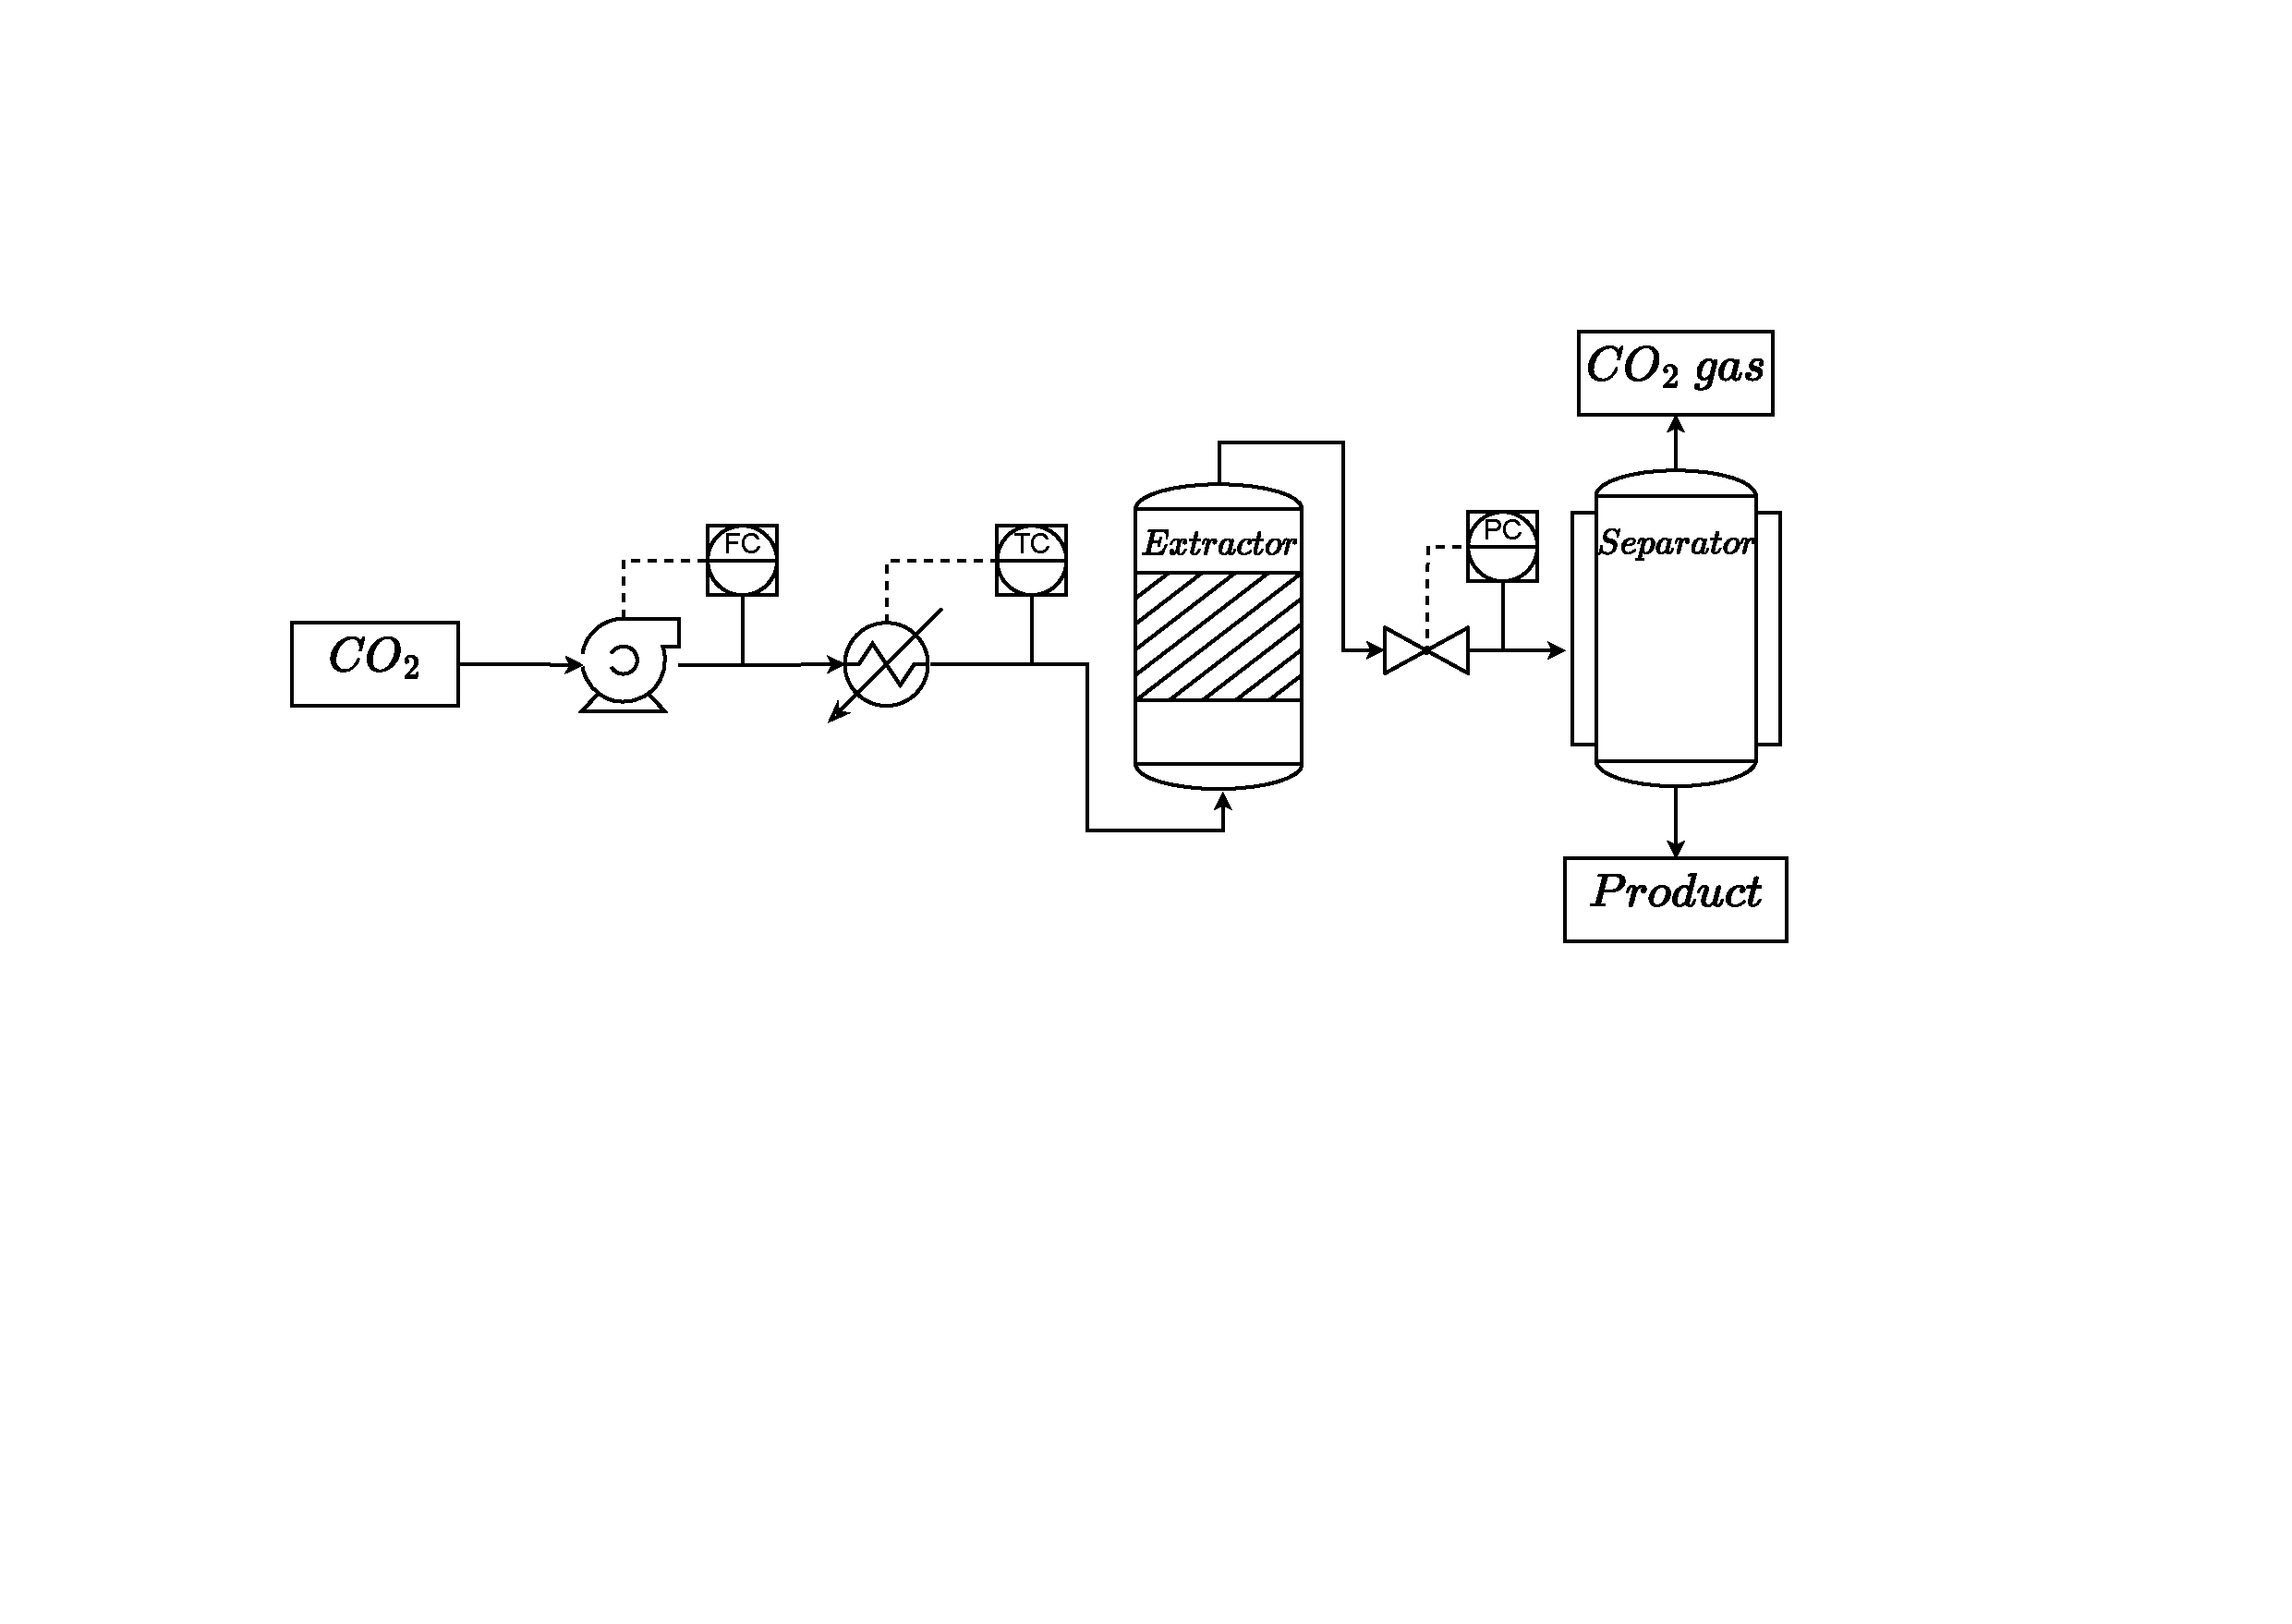
\includegraphics[trim = 5cm 12cm 8cm 6cm, clip,width=\columnwidth]{Figures/PFD.pdf}
		\caption{Process flow diagram}
		\label{fig: SFE_drawing}
	\end{figure}

	The purpose of this study is to develop a process model for the extraction of natural substances from solid materials and liquids using supercritical fluids, specifically supercritical $CO_2$. To achieve this, the model parameters are estimated based on thermodynamic relations and a set of experiments conducted at various conditions. The maximum likelihood estimator is used to solve the parameter estimation problem, and the obtained parameters are subjected to regression to derive correlations. These correlations enable the process model to be generalized across a range of temperatures (40 to $50^\circ C$) and pressures (200 to 300 bars).
	
	The study is structured as follows: Chapter \ref{CH: Thermodynamic} provides a general discussion on supercritical fluids to familiarize the reader with their properties. Chapter \ref{CH:Governing_equations_chapter} introduces the general balance equations, which are derived under the assumption of Low-Mach number in Chapter \ref{CH:Low_Mach_chapter}. The simplified balance equations are combined with the extraction kinetic equation to develop the process model in Chapter \ref{CH: Extraction_model}. The maximum likelihood technique is presented in Chapter \ref{CH: Parameter_estimation} and is then combined with the process model. The dataset obtained from laboratory experiments is used to close the optimization problem in Chapter \ref{CH: Experiments}. Finally, Chapters \ref{CH: Results} and \ref{CH: Conclusion} discuss the results of the parameter estimations and simulation results.
		
\end{document}